\documentclass[11pt]{article}
\usepackage[margin=1in]{geometry}
\usepackage[T1]{fontenc}
\usepackage[utf8]{inputenc}
\usepackage{lmodern}
\usepackage{amsmath,amssymb,amsthm}
\usepackage{booktabs}
\usepackage{hyperref}
\usepackage{enumitem}
\usepackage{listings}
\usepackage{url}
\usepackage{graphicx}
\usepackage{xcolor}
\usepackage[numbers]{natbib}
\usepackage{tikz}
\usetikzlibrary{arrows.meta,positioning,shapes.geometric,fit}

\hypersetup{
  colorlinks=true,
  linkcolor=blue,
  citecolor=blue,
  urlcolor=blue,
}

\lstset{
  basicstyle=\ttfamily\small,
  frame=single,
  breaklines=true,
  columns=fullflexible,
  keywordstyle=\color{blue},
  commentstyle=\color{gray},
  stringstyle=\color{red!70!black},
}

\newtheorem{definition}{Definition}
\newtheorem{proposition}{Proposition}
\newtheorem{remark}{Remark}

\title{Hallucination Is All You Need:\\
From Bash as Interface to Intent as Infrastructure\\
in LLM Agent Systems}

\author{
  Zhicong Liu \\
  OpenDAN / BuckyOS Project \\
  \texttt{liuzhicong@buckyos.org}
}
\date{March 2026}

\begin{document}
\maketitle

% ============================================================
\begin{abstract}
% ============================================================
Tool use in large language model (LLM) agents is conventionally framed as a \emph{schema exposure} problem: the system must inform the model which tools exist before the model can invoke them.
This shared assumption underpins four dominant paradigms---schema stuffing, select-then-call routing, minimal shell primitives, and interpreter-first code generation---each trading prompt overhead against capability breadth.
We challenge this assumption by observing that when an LLM emits a command or function call that does not exist in the current environment, the resulting failure is not merely an error but a \emph{high-quality, context-grounded declaration of intent}.

We present \textbf{Intent Engine}, a fifth tool-use paradigm that reinterprets LLM hallucinations as first-class intent signals.
In this architecture, the agent runtime injects zero tool schemas into the model's context window. Instead, the model expresses actions freely through a shell-centric interface.
When a command does not resolve, the runtime captures the unresolved invocation as a structured intent object, suspends the session, dispatches the intent to a separate \emph{realization agent} that synthesizes a thin executable wrapper from available system resources, and resumes the original session upon completion.
Bash serves not as a pre-registered tool but as a \emph{universal intent surface}---a compressed, compositional language through which the model's implicit knowledge is projected into actionable proposals.

We formalize the intent object model, the two-loop session architecture, the realization function, and the session-scoped lifecycle with natural decay semantics.
We provide an information-theoretic argument for why zero-schema injection maximizes the model's effective attention budget for task reasoning.
We analyze token cost, latency profiles, and safety boundaries, and ground the design in an existing implementation substrate---the OpenDAN/BuckyOS agent runtime---that already provides resumable sessions, persistent shell execution, and wait/resume control flow.
As the system is under active development, this paper presents the theoretical framework and architectural design rather than empirical benchmarks, which are deferred to a forthcoming companion report.
\end{abstract}

% ============================================================
\section{Introduction}
\label{sec:intro}
% ============================================================

The rapid advance of large language models has created a new class of software system: the \emph{LLM agent}, a program that combines language understanding with environment action to accomplish tasks on behalf of a user.
Whether the task is software engineering~\citep{sweagent2024,openhands2024}, system administration, personal productivity, or web interaction, the agent must convert a natural-language objective into a sequence of concrete environment operations.

The dominant engineering response has been to enrich the model with more tool specifications, better function schemas, or more elaborate tool routers~\citep{toolformer2023,gorilla2023,qin2024toolllm}.
This family of solutions treats tool invocation as fundamentally a \emph{closed-world interface design} problem: the system defines a fixed capability boundary and asks the model to operate within it.
This framing has achieved practical success, but it imposes inherent constraints on scalability, attention efficiency, and the ability to handle novel or unanticipated capabilities.

Recent engineering practice has demonstrated a striking alternative.
Terminal-native agents built around a minimal set of shell primitives---\texttt{bash}, \texttt{read\_file}, \texttt{write\_file}, \texttt{edit\_file}---have proven remarkably effective~\citep{sweagent2024,shihipar2026bash}.
The phrase ``Bash is all you need'' captures this insight: a single \texttt{exec\_bash} entry point activates an enormous reservoir of implicit knowledge that the model acquired during pre-training---knowledge about command-line tools, software conventions, Unix composition patterns, and real-world system administration.
This reservoir is far larger than what could be injected through explicit tool schemas.

We extend this insight one step further.
If bash is already the most natural action surface for coding-capable LLMs, then what happens when the model emits a bash command that \emph{does not exist}?
The conventional answer is: it is a hallucination, an error to be caught and reported back so the model can try again.
We argue for a different interpretation:

\begin{quote}
\textbf{A plausible but unresolved command emitted by an LLM is not merely an execution failure---it is a compact, context-grounded declaration of what capability the model believes should exist.}
\end{quote}

This reinterpretation motivates \textbf{Intent Engine}, a fifth tool-use paradigm.
Instead of telling the model what tools are available (schema exposure), Intent Engine lets the model express what tools it \emph{needs} (intent declaration) and asks the system to realize those tools on demand.
The hallucination becomes the specification.

\paragraph{Contributions.}
This paper makes the following contributions:
\begin{enumerate}[leftmargin=*]
  \item \textbf{A conceptual reframing}: we reinterpret unresolved LLM tool calls as first-class intent objects rather than ordinary execution failures, establishing a theoretical basis for treating hallucination as a productive system signal (\S\ref{sec:insight}).
  \item \textbf{A two-loop architecture}: we propose Intent Engine, a runtime design that separates \emph{session reasoning} from \emph{intent realization}, with bash as a universal intent surface and session-scoped capability lifecycle (\S\ref{sec:architecture}).
  \item \textbf{A formal framework}: we define intent objects, realization functions, session state machines, and provide token-cost and attention-efficiency analyses (\S\ref{sec:formalization}).
  \item \textbf{An implementation grounding}: we show how the architecture maps onto existing runtime primitives in the OpenDAN/BuckyOS agent platform (\S\ref{sec:implementation}).
  \item \textbf{A research agenda}: we articulate testable hypotheses, proposed benchmarks, and safety considerations for future empirical validation (\S\ref{sec:evaluation}).
\end{enumerate}

\paragraph{Scope and positioning.}
This is a \emph{systems and theory} paper.
The Intent Engine system is under active development; we present the design framework, formal analysis, and architectural blueprint rather than completed benchmark results.
We are explicit about what is implemented versus proposed, and we outline the experimental agenda that a forthcoming companion report will address.

% ============================================================
\section{Background: Four Tool-Use Paradigms}
\label{sec:background}
% ============================================================

Before introducing Intent Engine, we survey the four existing paradigms for equipping LLM agents with tool-use capabilities.
All four share a common structural assumption: \emph{the system must expose the tool inventory to the model before the model can act}.

\subsection{Schema Stuffing}
\label{sec:schema-stuffing}

The most direct approach injects the complete catalog of tool schemas---typically as JSON function definitions---into the model's system prompt or context window.
This works well at small scale (3--5 tools) but scales poorly.
As the tool inventory grows, prompt budget is consumed by interface descriptions rather than task-specific reasoning state, and the model's attention is diluted across rarely relevant tool definitions.

Let $n$ be the number of tools and $\bar{s}$ the average schema token length.
The prompt-side tool cost is $T_s = n \cdot \bar{s}$, which grows linearly and can easily consume thousands of tokens in real-world systems with dozens of tools.

\subsection{Select-then-Call}
\label{sec:select-then-call}

Router-based and retrieval-augmented systems address prompt bloat by separating tool \emph{selection} from tool \emph{execution}~\citep{toolformer2023,gorilla2023}.
In the simplest form, the agent first calls a \texttt{list\_tools} meta-function, selects the relevant tool from compressed descriptions, and then receives that tool's full schema in a subsequent turn.
This reduces the per-turn schema load from $O(n)$ to $O(1)$ tools, but doubles the number of LLM reasoning rounds per tool use.
The selection step itself introduces an additional error surface: the model must choose from brief descriptions without grounded execution context.

\subsection{Minimal Primitives: Bash is All You Need}
\label{sec:minimal-primitives}

A third approach, validated by agents such as SWE-agent~\citep{sweagent2024} and Claude Code~\citep{shihipar2026bash}, exposes only a handful of high-leverage primitives: typically \texttt{bash}, \texttt{read\_file}, \texttt{write\_file}, and \texttt{edit\_file}.
By treating the file system as a state machine and the shell as a compositional gateway, the agent relies on the model's implicit pre-training knowledge of command-line tools, package managers, compilers, and system utilities.

This paradigm reveals a fundamental insight: \emph{the action space reachable through a single \texttt{exec\_bash} primitive is vastly larger than what any explicit tool schema set could enumerate}.
The model's internal knowledge of bash commands, flags, pipes, and scripting patterns constitutes an enormous implicit tool inventory that requires zero prompt injection to activate.

\subsection{Interpreter-First: Everything is Code}
\label{sec:interpreter-first}

The fourth paradigm asks the model to bypass tool abstractions entirely and solve tasks by generating and executing code, typically Python.
This is maximally flexible---any computable function is in principle reachable---but it offloads even trivial operations into a full plan-code-compile-test-debug cycle.
For a simple intent like ``check the weather,'' requiring the model to construct an HTTP client, parse JSON responses, and handle errors is an inefficient use of the model's attention and reasoning budget.

\subsection{The Shared Assumption}
\label{sec:shared-assumption}

Despite their differences, all four paradigms share a structural presupposition:

\begin{quote}
\emph{The model must know what tools exist before it can invoke them.}
\end{quote}

Schema stuffing injects all schemas upfront.
Select-then-call reveals schemas on demand through a routing step.
Minimal primitives hardcode a small, fixed set.
Interpreter-first implicitly assumes that the model's code-generation capability \emph{is} the tool.
In every case, the capability boundary is defined by the system and presented to the model.

Intent Engine challenges this assumption.

% ============================================================
\section{Core Insight: Hallucination as Intent}
\label{sec:insight}
% ============================================================

\subsection{Observing LLM Behavior in the Wild}

A consistent empirical observation across diverse agent deployments is that LLMs frequently emit commands or function calls that do not correspond to any registered tool in the current environment.
The model might type \texttt{get\_weather cupertino} in a shell that has no weather utility installed, or invoke \texttt{search\_database(query="recent orders")} when no such function has been defined.

The standard engineering response is to treat these as \emph{hallucination errors}: the system returns an error message (e.g., \texttt{command not found}), the model observes the failure, and it attempts an alternative approach.
This error-and-retry loop is functional but wasteful---it discards information that the model has already computed.

\subsection{Reinterpreting Failed Invocations}

We propose a different reading.
When a model emits \texttt{get\_weather cupertino}, it has performed contextual reasoning and arrived at a conclusion: ``the current task requires weather information for Cupertino, and the most natural way to obtain it is through a command with this name and argument structure.''
The model does not need to \emph{know} whether \texttt{get\_weather} exists.
It is expressing an \emph{intent}---a compressed representation of what capability it believes should be available.

This reinterpretation is supported by three observations:

\begin{enumerate}[leftmargin=*]
  \item \textbf{Plausibility}: LLM-generated commands are overwhelmingly plausible. The command names are descriptive, the argument structures follow conventions, and the invocations are contextually appropriate. This is a direct consequence of pre-training on vast corpora of real command-line usage, API documentation, and software engineering discourse.

  \item \textbf{Compression}: a shell command is an extremely compressed intent representation. The command name encodes the desired action, the arguments encode the parameters, and the expected output format is implicitly constrained by shell conventions (text to stdout). This is far more token-efficient than an equivalent natural-language description of the same intent.

  \item \textbf{Consistency}: across different sessions and contexts, models tend to generate similar command structures for similar intents, suggesting that these ``hallucinations'' are not random noise but reflect stable learned patterns about how capabilities should be named and parameterized.
\end{enumerate}

\subsection{From Error Signal to System Input}

The philosophical shift is summarized as follows:

\begin{quote}
\textbf{Don't tell the LLM what it can do. Let it tell you what it wants to do.}
\end{quote}

In traditional tool-use architectures, information flows from the system to the model: ``here are your available tools.''
In Intent Engine, information flows from the model to the system: ``here is what I need.''
The hallucination is not a bug to be corrected; it is the model's \emph{proposal} for what the tool interface should look like.
The system's job is to decide whether and how to realize that proposal.

This inversion has a direct parallel in programming language design: the distinction between \emph{nominal typing} (you must declare the interface before using it) and \emph{structural typing} (the system infers the interface from usage).
Intent Engine applies structural typing to tool invocation.

% ============================================================
\section{Intent Engine: Architecture}
\label{sec:architecture}
% ============================================================

\subsection{Design Principles}

Intent Engine is guided by four principles:

\begin{enumerate}[leftmargin=*]
  \item \textbf{Zero schema injection}: the main LLM session receives no tool schemas in its context window. All attention budget is reserved for task reasoning.
  \item \textbf{Hallucination as specification}: unresolved commands are captured as structured intent objects rather than discarded as errors.
  \item \textbf{Separation of concerns}: task reasoning (main session) and capability synthesis (realization agent) operate in separate loops with distinct context windows.
  \item \textbf{Ephemeral realization}: synthesized capabilities are session-scoped, avoiding global state pollution and enabling natural evolution.
\end{enumerate}

\subsection{Two-Loop Architecture}
\label{sec:two-loop}

Intent Engine consists of two concurrent processing loops (Figure~\ref{fig:architecture}).

\paragraph{Loop 1: Main session.}
The primary LLM session receives user input, performs task reasoning, and emits actions through a shell-centric interface.
Actions that resolve in the current environment execute immediately, and their results flow back into the conversation.
When an action fails because the command does not exist, instead of returning \texttt{command not found}, the runtime:
\begin{enumerate}[leftmargin=*]
  \item captures the full invocation context (command, arguments, surrounding conversation, session policy),
  \item constructs a structured intent object,
  \item suspends the session in a \texttt{WAIT} state,
  \item enqueues the intent for realization.
\end{enumerate}

\paragraph{Loop 2: Intent realization.}
A separate agent (or specialized runtime service) consumes intents from the queue.
For each intent, it examines the command surface form, parsed arguments, session context, available system resources (APIs, SDKs, packages, services), and applicable policy constraints.
It then selects one of three outcomes:

\begin{description}[leftmargin=*]
  \item[\texttt{REALIZE}:] Synthesize a thin wrapper script that fulfills the intent by bridging to existing system capabilities. Install the wrapper into the session-local executable namespace.
  \item[\texttt{REJECT}:] Determine that the intent violates policy, exceeds authority bounds, or cannot be safely realized. Return a structured explanation to the main session.
  \item[\texttt{ESCALATE}:] The intent is realizable but requires human approval, additional credentials, or capability installation beyond the agent's authority. Suspend until approval is granted.
\end{description}

Upon successful realization, the runtime resumes the main session, which re-executes the originally failed command---now finding the newly installed wrapper---and continues its task.

\begin{figure}[t]
\centering
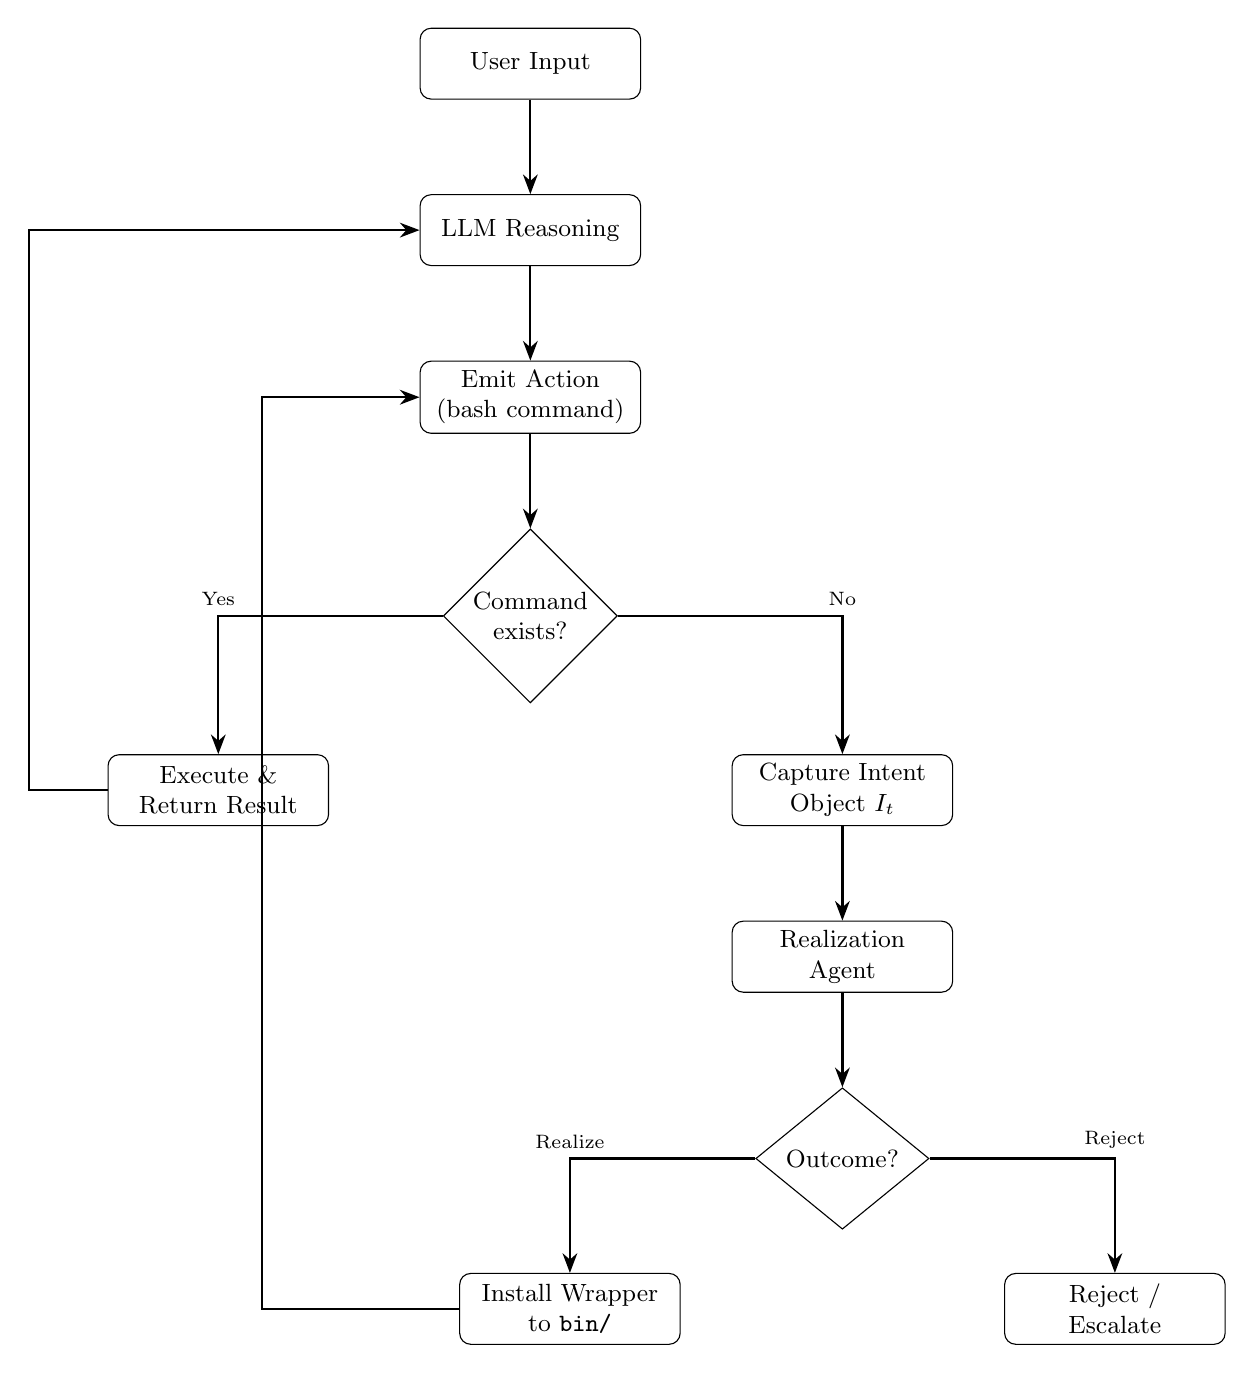
\begin{tikzpicture}[
  node distance=1.2cm and 2.5cm,
  box/.style={draw, rounded corners, minimum width=2.8cm, minimum height=0.9cm, align=center, font=\small},
  decision/.style={draw, diamond, minimum width=2.2cm, minimum height=1.2cm, align=center, font=\small, inner sep=1pt},
  arrow/.style={-{Stealth[length=2.5mm]}, thick},
]
  \node[box] (user) {User Input};
  \node[box, below=of user] (llm) {LLM Reasoning};
  \node[box, below=of llm] (action) {Emit Action\\(bash command)};
  \node[decision, below=of action] (exists) {Command\\exists?};
  \node[box, below left=1.2cm and 2.0cm of exists] (exec) {Execute \&\\Return Result};
  \node[box, below right=1.2cm and 2.0cm of exists] (capture) {Capture Intent\\Object $I_t$};
  \node[box, below=of capture] (realize) {Realization\\Agent};
  \node[decision, below=of realize] (outcome) {Outcome?};
  \node[box, below left=1.0cm and 1.5cm of outcome] (install) {Install Wrapper\\to \texttt{bin/}};
  \node[box, below right=1.0cm and 1.5cm of outcome] (reject) {Reject /\\Escalate};

  \draw[arrow] (user) -- (llm);
  \draw[arrow] (llm) -- (action);
  \draw[arrow] (action) -- (exists);
  \draw[arrow] (exists) -| node[above,font=\scriptsize]{Yes} (exec);
  \draw[arrow] (exists) -| node[above,font=\scriptsize]{No} (capture);
  \draw[arrow] (exec.west) -- ++(-1.0,0) |- (llm.west);
  \draw[arrow] (capture) -- (realize);
  \draw[arrow] (realize) -- (outcome);
  \draw[arrow] (outcome) -| node[above,font=\scriptsize]{Realize} (install);
  \draw[arrow] (outcome) -| node[above,font=\scriptsize]{Reject} (reject);
  \draw[arrow] (install.west) -- ++(-2.5,0) |- (action.west);
\end{tikzpicture}
\caption{Two-loop architecture of Intent Engine. The main session loop (left path) handles normal execution. The realization loop (right path) captures unresolved commands, synthesizes wrappers, and resumes the session.}
\label{fig:architecture}
\end{figure}

\subsection{Bash as Universal Intent Surface}
\label{sec:bash-surface}

Intent Engine uses bash as its primary action language. This choice is not arbitrary; it reflects three structural advantages of shell commands as an intent representation:

\begin{enumerate}[leftmargin=*]
  \item \textbf{Action naming}: the command token itself encodes the desired capability (e.g., \texttt{get\_weather}, \texttt{resize\_image}, \texttt{deploy\_service}).
  \item \textbf{Argument structure}: positional arguments and flags provide a lightweight, convention-rich parameter schema (e.g., \texttt{--city cupertino --unit celsius}).
  \item \textbf{Compositionality}: pipes, redirection, subshells, and command chaining allow complex intents to be expressed as compositions of simpler ones.
\end{enumerate}

Compared with JSON-formatted function calls (the format used by most tool-calling APIs), bash commands are:
\begin{itemize}[leftmargin=*]
  \item more \emph{token-efficient}: \texttt{get\_weather cupertino} vs.\ \texttt{\{"name": "get\_weather", "arguments": \{"location": "cupertino"\}\}},
  \item more \emph{aligned with model priors}: LLMs have been trained on orders of magnitude more shell transcripts than JSON function-call schemas,
  \item more \emph{compositionally expressive}: a pipe like \texttt{get\_weather cupertino | format\_json} expresses a two-step intent in a single line.
\end{itemize}

The phrase ``Bash is all you need''~\citep{shihipar2026bash} captures the insight that shell access alone unlocks a vast implicit capability space.
Intent Engine extends this to: \emph{even when a bash command doesn't exist, the attempt to call it is itself a useful interface specification}.

\subsection{Session-Scoped Realization and Natural Decay}
\label{sec:lifecycle}

Realized intents follow a session-scoped lifecycle:

\begin{enumerate}[leftmargin=*]
  \item \textbf{Instantiation}: The model's first unresolved invocation triggers the realization loop. A wrapper is synthesized and installed in the session-local \texttt{bin/} directory (prepended to the session's \texttt{PATH}).

  \item \textbf{Reuse}: Subsequent calls to the same command within the session resolve directly via the installed wrapper---zero additional LLM reasoning, zero realization latency.

  \item \textbf{Decay}: When the session ends, or when the conversation context rolls past the point where the command was established, the wrapper is removed. The capability ceases to exist.

  \item \textbf{Reinstantiation}: In a future session, if the model again needs the same capability, it will naturally emit a similar command. The realization loop fires again, potentially producing an \emph{improved} wrapper (because the underlying system resources may have changed).
\end{enumerate}

This lifecycle is deliberate, not a caching failure. It provides:
\begin{itemize}[leftmargin=*]
  \item \textbf{Scope isolation}: different sessions can have different tool sets without global namespace conflicts.
  \item \textbf{Freshness}: wrappers are always built against the current state of system resources, avoiding staleness.
  \item \textbf{Minimal management}: no tool registry, no version tracking, no deprecation workflow.
\end{itemize}

The analogy is to \emph{just-in-time compilation}: capabilities are materialized when needed, used while hot, and discarded when the execution context ends.

% ============================================================
\section{Formalization}
\label{sec:formalization}
% ============================================================

\subsection{Intent Objects}

\begin{definition}[Intent Object]
An intent object is a tuple $I_t = \langle s_t,\, \alpha_t,\, x_t,\, p_t,\, d_t \rangle$ where:
\begin{itemize}[leftmargin=*]
  \item $s_t$ is the \emph{surface form}: the raw string emitted by the model (e.g., \texttt{get\_weather cupertino}),
  \item $\alpha_t = (\textit{cmd},\, \textit{args})$ is the \emph{parsed structure}: command name and argument list extracted from $s_t$,
  \item $x_t$ is the \emph{context bundle}: relevant conversation history, task description, and environment state at time $t$,
  \item $p_t$ is the \emph{policy profile}: security constraints, authority bounds, and resource limits applicable to the current session,
  \item $d_t \in \mathbb{R}^+$ is the \emph{deadline budget}: maximum time allowed for realization before the session times out.
\end{itemize}
\end{definition}

\subsection{Realization Function}

\begin{definition}[Realization Function]
The realization function maps an intent object, the current capability set, and the environment state to an outcome:
\[
R: \mathcal{I} \times \mathcal{C} \times \mathcal{E} \rightarrow \{\texttt{wrapper}(w),\; \texttt{reject}(r),\; \texttt{escalate}(e)\}
\]
where:
\begin{itemize}[leftmargin=*]
  \item $\mathcal{I}$ is the space of intent objects,
  \item $\mathcal{C}$ is the current set of available system capabilities (APIs, packages, services),
  \item $\mathcal{E}$ is the environment state (filesystem, network, sandbox configuration),
  \item $w$ is an executable wrapper, $r$ is a rejection reason, and $e$ is an escalation request.
\end{itemize}
\end{definition}

A successful wrapper $w$ must satisfy three properties:

\begin{proposition}[Wrapper Correctness]
A wrapper $w$ produced by $R(I_t, C, E) = \texttt{wrapper}(w)$ is correct if and only if:
\begin{enumerate}[leftmargin=*]
  \item \textbf{Surface compatibility}: $w$ accepts the invocation form specified by $s_t$ and $\alpha_t$.
  \item \textbf{Policy conformance}: the execution of $w$ does not exceed the authority bounds defined by $p_t$.
  \item \textbf{Semantic fidelity}: the output of $w$ fulfills the intent implied by $x_t$ as judged against the task context.
\end{enumerate}
\end{proposition}

\subsection{Session State Machine}

\begin{definition}[Session States]
A session $\sigma$ transitions through the following states:
\[
\sigma \in \{\texttt{READY},\; \texttt{RUNNING},\; \texttt{WAIT}(I_t),\; \texttt{END}\}
\]
with transitions:
\begin{align}
\texttt{READY} &\xrightarrow{\text{user input}} \texttt{RUNNING} \label{eq:t1}\\
\texttt{RUNNING} &\xrightarrow{\text{action resolves}} \texttt{READY} \label{eq:t2}\\
\texttt{RUNNING} &\xrightarrow{\text{action unresolved}} \texttt{WAIT}(I_t) \label{eq:t3}\\
\texttt{WAIT}(I_t) &\xrightarrow{R(I_t) = \texttt{wrapper}} \texttt{RUNNING} \label{eq:t4}\\
\texttt{WAIT}(I_t) &\xrightarrow{R(I_t) = \texttt{reject}} \texttt{READY}\;\text{(with error)} \label{eq:t5}\\
\texttt{WAIT}(I_t) &\xrightarrow{\text{timeout}(d_t)} \texttt{READY}\;\text{(with fallback)} \label{eq:t6}\\
\texttt{RUNNING} &\xrightarrow{\text{task complete}} \texttt{END} \label{eq:t7}
\end{align}
\end{definition}

The key novelty is transition~\eqref{eq:t3}$\to$\eqref{eq:t4}: an unresolved action triggers suspension rather than immediate error propagation, creating a window for asynchronous capability synthesis.

\subsection{Token Cost Analysis}
\label{sec:token-analysis}

Let us compare the prompt-side token costs across paradigms for a system with $n$ available tools, of which $k \ll n$ are used in a given session.

\begin{table}[h]
\centering
\caption{Prompt-side token cost per paradigm. $\bar{s}$: average schema tokens per tool. $\bar{d}$: average description tokens for routing. $T_{\text{prim}}$: tokens for primitive tool definitions (typically $<100$).}
\label{tab:token-cost}
\begin{tabular}{lcc}
\toprule
\textbf{Paradigm} & \textbf{Per-turn schema tokens} & \textbf{Per-use LLM rounds} \\
\midrule
Schema stuffing & $n \cdot \bar{s}$ & 1 \\
Select-then-call & $n \cdot \bar{d} + \bar{s}$ & 2 \\
Minimal primitives & $T_{\text{prim}}$ (constant) & 1 \\
Interpreter-first & $\approx 0$ (code prompt) & 1+ (debug loop) \\
\textbf{Intent Engine} & $\mathbf{0}$ & 1 (after realization) \\
\bottomrule
\end{tabular}
\end{table}

Intent Engine achieves zero prompt-side tool token cost because no schema is injected into the main session's context.
The realization cost is paid in a separate context window by the realization agent, which does not burden the main session's attention budget.

\subsection{Attention Efficiency Argument}
\label{sec:attention}

Modern transformer-based LLMs allocate attention across all tokens in the context window.
When tool schemas consume a fraction $\frac{T_s}{T_{\text{total}}}$ of the context, the remaining $\frac{T_{\text{total}} - T_s}{T_{\text{total}}}$ is available for task-relevant reasoning.

\begin{proposition}[Attention Budget]
For a context window of size $T_{\text{total}}$, the effective task attention $A_{\text{task}}$ satisfies:
\[
A_{\text{task}} \propto 1 - \frac{T_{\text{schema}}}{T_{\text{total}}}
\]
where $T_{\text{schema}}$ is the token count consumed by tool definitions.
Intent Engine sets $T_{\text{schema}} = 0$, maximizing $A_{\text{task}}$.
\end{proposition}

This is not merely a theoretical argument.
In practice, agents with large tool inventories (50+ tools) can dedicate 20--40\% of their context window to schema definitions~\citep{qin2024toolllm}.
This creates a direct tradeoff: more tools available means less context for the actual task.
Intent Engine eliminates this tradeoff entirely.

\subsection{Latency Profile}
\label{sec:latency}

Intent Engine has a distinctive latency profile:

\begin{itemize}[leftmargin=*]
  \item \textbf{First-use latency $L_f$}: High. The realization loop must synthesize, test, and install a wrapper. This may involve a secondary LLM call, code generation, and validation.
  \item \textbf{Repeated-use latency $L_r$}: Low. The wrapper is a local executable; invocation is a standard process spawn with no LLM overhead.
  \item \textbf{Amortized latency}: For an intent invoked $m$ times in a session:
  \[
  L_{\text{amortized}} = \frac{L_f + (m-1) \cdot L_r}{m} \xrightarrow{m \to \infty} L_r
  \]
\end{itemize}

The architecture is therefore most advantageous in sessions where:
\begin{enumerate}[leftmargin=*]
  \item the tool space is large or unbounded,
  \item capabilities are reused within a session,
  \item wrappers are thin (bridging to existing APIs rather than implementing complex logic from scratch).
\end{enumerate}

% ============================================================
\section{Comparison with Existing Paradigms}
\label{sec:comparison}
% ============================================================

Table~\ref{tab:comparison} provides a systematic comparison across six dimensions.

\begin{table}[h]
\centering
\caption{Multi-dimensional comparison of tool-use paradigms.}
\label{tab:comparison}
\small
\begin{tabular}{@{}lccccc@{}}
\toprule
\textbf{Dimension} & \textbf{Schema} & \textbf{Select-} & \textbf{Minimal} & \textbf{Interpreter} & \textbf{Intent} \\
 & \textbf{Stuffing} & \textbf{then-Call} & \textbf{Primitives} & \textbf{First} & \textbf{Engine} \\
\midrule
Prompt overhead & High & Medium & Low & Low & \textbf{Zero} \\
Attention efficiency & Low & Medium & High & Medium & \textbf{Highest} \\
Tool scalability & Poor & Medium & Ecosystem & Good & \textbf{Unbounded} \\
First-use latency & Low & High & Low & High & High \\
Repeated-use latency & Low & High & Low & High & \textbf{Low} \\
Implementation cost & Low & Medium & Low & Medium & High \\
\bottomrule
\end{tabular}
\end{table}

Intent Engine's unique position is the combination of zero prompt overhead with unbounded tool scalability.
No other paradigm achieves both simultaneously.
The cost is implementation complexity and first-use latency, which we argue is an acceptable tradeoff for systems that operate in large, evolving capability spaces.

\paragraph{Relationship to minimal primitives.}
Intent Engine is best understood as an \emph{extension} of the minimal-primitives paradigm, not a replacement.
The ``Bash is all you need'' insight~\citep{shihipar2026bash} established that shell access alone is sufficient for many tasks.
Intent Engine adds: when shell access encounters a gap, the gap itself is informative and actionable.
The two approaches are complementary and can coexist in the same runtime.

% ============================================================
\section{Implementation Substrate: OpenDAN/BuckyOS}
\label{sec:implementation}
% ============================================================

The Intent Engine design is grounded in the OpenDAN/BuckyOS agent runtime, which provides several primitives that map directly onto the architecture's requirements.

\subsection{Resumable Session State}

The runtime implements sessions as explicit state machines with persistent records.
Sessions can enter \texttt{Wait} states with associated metadata, resume upon external events, and enforce timeout-driven fallback transitions.
This is precisely the control-plane primitive needed for intent suspension and resumption (transitions~\eqref{eq:t3}--\eqref{eq:t6}).

\subsection{Persistent Shell Execution}

The runtime provides a persistent \texttt{exec\_bash} capability that maintains per-session working-directory continuity and long-lived shell context.
This gives Intent Engine a natural observation surface: unresolved commands can be detected, and the session-local \texttt{PATH} can be dynamically extended with realized wrappers.

\subsection{Worklog and Action Arbitration}

The runtime includes worklog recording, expectation management, and action arbitration infrastructure.
These provide the audit trail and policy enforcement layers that Intent Engine requires for safe operation.

\subsection{Implementation Status}

We distinguish clearly between what exists and what is proposed:

\begin{itemize}[leftmargin=*]
  \item \textbf{Implemented}: Session lifecycle management, wait/resume semantics, persistent bash execution, tool registration framework, action logging.
  \item \textbf{Proposed}: Automatic detection of unresolved commands as intent objects, semantic normalization pipeline, wrapper synthesis via realization agent, policy-constrained realization, cross-session intent analytics.
\end{itemize}

The gap between implemented substrate and proposed intent layer is the primary focus of our ongoing engineering effort.

% ============================================================
\section{Illustrative Walkthrough}
\label{sec:example}
% ============================================================

We present a concrete scenario to illustrate the full lifecycle.

\paragraph{Step 1: User request.}
The user asks: ``What's the weather like in Cupertino today?''

\paragraph{Step 2: LLM reasoning.}
The main session LLM, with no tool schemas in its context, reasons about the task and determines that weather data is needed. Drawing on its pre-training knowledge, it emits:

\begin{lstlisting}
$ get_weather cupertino
\end{lstlisting}

\paragraph{Step 3: Intent capture.}
The runtime detects that \texttt{get\_weather} is not in the current \texttt{PATH}. Instead of returning \texttt{command not found}, it constructs:
\[
I_t = \langle \texttt{"get\_weather cupertino"},\; (\texttt{get\_weather}, [\texttt{cupertino}]),\; x_t,\; p_t,\; 30\text{s} \rangle
\]
The session enters \texttt{WAIT}($I_t$).

\paragraph{Step 4: Realization.}
The realization agent examines the intent, discovers that the system has a weather API SDK installed (\texttt{tools.weather\_api}), and synthesizes a wrapper:

\begin{lstlisting}[language=Python]
#!/usr/bin/env python3
# Session-local wrapper: ~/.session/bin/get_weather
# Auto-generated by Intent Engine realization agent
import sys
from tools.weather_api import fetch_weather

location = sys.argv[1] if len(sys.argv) > 1 else "unknown"
result = fetch_weather(location=location, unit="celsius")
print(f"{result['location']}: {result['temp']}C, "
      f"{result['condition']}")
\end{lstlisting}

The wrapper is installed as an executable in the session's \texttt{bin/} directory.

\paragraph{Step 5: Resume.}
The session resumes and re-executes \texttt{get\_weather cupertino}. The command now resolves, returning formatted weather data. The LLM incorporates the result and responds to the user.

\paragraph{Step 6: Reuse.}
Later in the session, the user asks about weather in another city. The LLM emits \texttt{get\_weather tokyo}. The command resolves immediately via the installed wrapper---no realization needed.

\paragraph{Step 7: Decay.}
When the session ends, the \texttt{bin/} directory is cleaned up. The \texttt{get\_weather} wrapper ceases to exist. In a future session, if the capability is needed again, it will be re-realized, potentially using updated APIs or improved synthesis.

\medskip

This example is intentionally simple. The architecture's true value emerges in scenarios with large, heterogeneous capability spaces---system administration, multi-service orchestration, data pipeline construction---where pre-registering every possible tool is infeasible.

% ============================================================
\section{Safety, Governance, and Failure Modes}
\label{sec:safety}
% ============================================================

The power of Intent Engine---an unbounded, dynamically generated tool space---is also its primary risk surface.
We identify four categories of concern.

\subsection{Intent Normalization}

Semantically equivalent intents may appear under different surface forms:
\begin{itemize}[leftmargin=*]
  \item \texttt{get\_weather cupertino}
  \item \texttt{weather cupertino}
  \item \texttt{check\_forecast --city cupertino}
  \item \texttt{forecast cupertino today}
\end{itemize}

Without normalization, each variant triggers a separate realization, wasting resources and creating redundant wrappers.
The realization agent must implement semantic deduplication, either through embedding-based similarity, canonical form mapping, or explicit aliasing after first realization.

\subsection{Authority Escalation}

A model-generated intent might request capabilities that exceed the session's authority---e.g., \texttt{delete\_all\_files /} or \texttt{send\_email ceo@company.com}.
The realization function must enforce \emph{policy-first} evaluation: check authority bounds before attempting synthesis.
This requires:
\begin{itemize}[leftmargin=*]
  \item explicit capability whitelists and blacklists per session,
  \item sandbox constraints on synthesized wrappers (filesystem scope, network access, resource limits),
  \item mandatory human escalation for sensitive operations.
\end{itemize}

\subsection{Wrapper Quality and Verification}

Synthesized wrappers are code generated by an LLM, and therefore subject to the usual risks of LLM-generated code: bugs, security vulnerabilities, incorrect API usage.
The realization loop should include:
\begin{itemize}[leftmargin=*]
  \item basic testing (dry-run with synthetic inputs),
  \item static analysis for common vulnerability patterns,
  \item output format validation against the intent specification.
\end{itemize}

\subsection{Latency and Timeout Handling}

If the realization agent cannot synthesize a wrapper within the deadline budget $d_t$, the system must degrade gracefully. Options include:
\begin{itemize}[leftmargin=*]
  \item returning a structured error explaining the capability gap,
  \item falling back to a natural-language description of what was attempted,
  \item suggesting an alternative action path.
\end{itemize}

The worst-case user experience occurs when realization is slow \emph{and} silent. The system should always provide progress feedback during the wait state.

% ============================================================
\section{Evaluation Agenda}
\label{sec:evaluation}
% ============================================================

Because the Intent Engine system is under active development, we present testable hypotheses and proposed evaluation methodology rather than completed benchmarks.

\subsection{Hypotheses}

\begin{description}[leftmargin=*,style=nextline]
  \item[H1: Prompt efficiency.] On tasks that use sparse subsets of a large tool inventory ($k \ll n$), Intent Engine will consume fewer prompt tokens than schema stuffing and select-then-call, with no degradation in task success rate.

  \item[H2: Repeated-use amortization.] After first realization, repeated invocations of the same capability will achieve lower end-to-end latency than select-then-call and interpreter-first approaches.

  \item[H3: Open-ended capability.] Intent Engine will outperform fixed-tool-inventory systems on tasks requiring novel capabilities that are absent from the pre-registered tool set but realizable from available system resources.

  \item[H4: Safety-governance coupling.] Without strong realization governance (sandbox constraints, policy enforcement, wrapper verification), unrestricted intent realization will exhibit higher security violation rates than closed-world tool systems.
\end{description}

\subsection{Proposed Benchmarks}

We propose three benchmark families:

\begin{enumerate}[leftmargin=*]
  \item \textbf{Sparse tool selection benchmark}: Tasks drawn from a catalog of $n \geq 100$ tools where each episode uses $k \leq 5$. Measures prompt efficiency and task success across paradigms.

  \item \textbf{Novel capability synthesis benchmark}: Tasks whose required capability is absent from the initial tool set but achievable through existing system packages and APIs. Measures the system's ability to synthesize correct wrappers without pre-registration.

  \item \textbf{Long-horizon reuse benchmark}: Multi-step sessions where the same capabilities are invoked repeatedly. Measures amortized latency and the benefit of session-local caching.
\end{enumerate}

\subsection{Metrics}

Key metrics include:
\begin{itemize}[leftmargin=*]
  \item prompt tokens consumed by tool exposure (per turn, per session),
  \item first-use and repeated-use latency (wall-clock time),
  \item task success rate (end-to-end task completion),
  \item realization success rate (fraction of intents successfully realized),
  \item wrapper reuse rate (cache hit ratio within session),
  \item normalization accuracy (semantic deduplication quality),
  \item safety violation rate under adversarial prompts.
\end{itemize}

% ============================================================
\section{Discussion}
\label{sec:discussion}
% ============================================================

\subsection{When Intent Engine is Not the Right Choice}

Intent Engine is not universally superior. It is poorly suited for:
\begin{itemize}[leftmargin=*]
  \item \textbf{Small, stable tool sets}: If the system has 3--5 well-defined tools, schema stuffing is simpler and incurs negligible attention cost.
  \item \textbf{Latency-critical single-shot tasks}: If the task requires exactly one tool call and latency is critical, the first-use realization cost is unacceptable.
  \item \textbf{Environments without a synthesis substrate}: If no APIs, packages, or services exist to bridge against, the realization agent has nothing to compose.
\end{itemize}

\subsection{Hybrid Architectures}

The most practical deployment may combine paradigms:
\begin{itemize}[leftmargin=*]
  \item A small set of \emph{core primitives} (bash, file operations) is always available---the minimal-primitives baseline.
  \item A \emph{frequently-used tool set} can be optionally pre-loaded via schema stuffing for latency-sensitive operations.
  \item Intent Engine handles the \emph{long tail}: rare, novel, or context-specific capabilities that are not worth pre-registering but can be realized on demand.
\end{itemize}

This hybrid approach captures the strengths of each paradigm where they are most appropriate.

\subsection{Implications for LLM Training}

If Intent Engine becomes a widely adopted pattern, it may influence how future LLMs are trained.
Models that are explicitly trained to emit well-structured intent commands---with consistent naming conventions, predictable argument patterns, and compositional structure---would be more effective in this architecture.
This suggests a co-evolutionary dynamic between agent runtime design and model training objectives.

\subsection{Beyond Tool Calling: Intent as a General Interface}

While this paper focuses on tool invocation, the intent-as-interface pattern may generalize.
Consider:
\begin{itemize}[leftmargin=*]
  \item \textbf{Knowledge intents}: the model asks for information it doesn't have, and the system retrieves it (a form of retrieval-augmented generation where the query is a shell-like command rather than a search string).
  \item \textbf{Communication intents}: the model expresses a desire to interact with another agent or service, and the runtime establishes the connection.
  \item \textbf{Configuration intents}: the model declares what environment properties it needs, and the system provisions them.
\end{itemize}

In each case, the pattern is the same: the model proposes an interface it wishes existed, and the system decides whether and how to provide it.

% ============================================================
\section{Related Work}
\label{sec:related}
% ============================================================

\paragraph{Reasoning and acting.}
ReAct~\citep{react2022} demonstrated that interleaving reasoning traces with actions improves both task performance and interpretability. Intent Engine extends this by treating failed actions as a new category of informative output rather than mere execution errors.

\paragraph{Self-supervised tool use.}
Toolformer~\citep{toolformer2023} showed that models can learn when and how to use tools through self-supervised training. While Toolformer focuses on learning to call existing tools, Intent Engine addresses the complementary problem of what happens when the needed tool does not yet exist.

\paragraph{API-scale tool grounding.}
Gorilla~\citep{gorilla2023} and ToolLLM~\citep{qin2024toolllm} tackled tool use at scale through retrieval-augmented API grounding, demonstrating that models can work with large tool inventories when augmented with retrieval. Intent Engine takes a different approach: instead of grounding the model's output in a known API catalog, it uses the model's output to \emph{define} what API should be created.

\paragraph{Agent-computer interfaces.}
SWE-agent~\citep{sweagent2024} showed the importance of carefully designed agent-computer interfaces for software engineering, emphasizing that interface design significantly affects agent performance. Intent Engine extends this insight by proposing that the interface can be dynamically generated rather than statically designed.

\paragraph{Shell-centric agent design.}
Recent engineering practice around terminal-native agents~\citep{shihipar2026bash} has validated that shell-centric action surfaces are highly effective for coding agents. The ``Bash is all you need'' philosophy established that a single shell entry point can activate vast implicit capabilities. Intent Engine builds directly on this foundation: bash is not just the interface, but the \emph{intent language}.

\paragraph{Dynamic tool creation.}
CREATOR~\citep{qian2023creator} explored the idea of LLMs creating tools during task solving, using a create-then-use pipeline. Intent Engine differs in its trigger mechanism (hallucination-driven rather than explicit creation instructions), its session-scoped lifecycle, and its use of bash as the universal surface form.

\paragraph{LLM hallucination as signal.}
While the broader literature on hallucination focuses on detection and mitigation~\citep{huang2023hallucination}, Intent Engine proposes the opposite for a specific domain: in tool invocation contexts, certain hallucinations carry structured semantic content that can be operationalized rather than suppressed.

\paragraph{Open-ended agent environments.}
Voyager~\citep{wang2023voyager} demonstrated that LLM agents can build a growing library of reusable skills in open-ended environments. Intent Engine shares the spirit of skill accumulation but differs in mechanism: skills are triggered by hallucinated commands rather than explicit curriculum learning, and they are session-scoped rather than persistent.

% ============================================================
\section{Conclusion}
\label{sec:conclusion}
% ============================================================

This paper advances a simple but consequential thesis: \textbf{in LLM agent systems, not every hallucinated command is a bug---some are compact, context-grounded declarations of what capability the model believes should exist.}

Intent Engine operationalizes this thesis through a two-loop architecture that separates task reasoning from capability synthesis, uses bash as a universal intent surface, and manages realized capabilities through a session-scoped lifecycle with natural decay.
The architecture achieves zero prompt-side tool cost, unbounded capability scalability, and amortized low latency for repeated use---at the expense of higher first-use latency and stronger requirements for safety governance.

The title ``Hallucination Is All You Need'' is deliberately provocative, echoing both the attention mechanism paper that launched the transformer era~\citep{vaswani2017attention} and the engineering maxim ``Bash is all you need''~\citep{shihipar2026bash} that established shell-centric agent design.
Our claim is narrower but precise: for the specific problem of tool invocation in agent systems, the model's tendency to invoke nonexistent capabilities is not a defect to be suppressed but a \emph{design resource} to be harnessed.

The question shifts from ``Which tools should we inject into the prompt?'' to ``How should we operationalize the model's proposed intents under policy and time constraints?''
We believe this shift opens a productive research direction at the intersection of agent architecture, runtime systems, and LLM behavior---one where the model's imperfections become a generative force rather than a liability.

\paragraph{Availability.}
The OpenDAN/BuckyOS runtime substrate is open-source.\footnote{\url{https://github.com/buckyos}} Experimental validation of the Intent Engine layer is in progress; benchmark results will be reported in a forthcoming companion paper.

% ============================================================
% References
% ============================================================

\bibliographystyle{plainnat}
\bibliography{intent_engine_references}

\end{document}
